\chapter{NVARs in Practice}\label{ch:nvar-application}

In this chapter, I will resolve the practical questions raised in
\cref{ch:nvar}, and demonstrate that NVARs are capable of solving
traditional RC problems well with very few taps, simple
nonlinearities, and very little training data. Using the example
systems from \cref{ch:systems}, I will use NVARs to perform state
inference and forecasting on the Lorenz '63 system, forecasting on the
double-scroll circuit, and forecasting on the Mackey-Glass time-delay
system.

The work presented in this chapter is the result of a
collaboration with Daniel~J.~Gauthier, Erik~Bollt, and Wendson~A.S.~Barbosa~\cite{gauthier2021}. My contribution involves the initial
implementation and exploration of the NVAR method, discussion during
the development of the Lorenz '63 results, as well as the
implementation of the Lorenz return map, double-scroll forecasting,
and Mackey-Glass forecasting.

\section{State Inference with Lorenz '63}

For this inference task, I provide an NVAR with the $x$ and $y$
components of the Lorenz '63 system, and train it to infer the third
$z$ variable. Inference tasks like this are useful in situations where
some variables of a system are easily measurable, while the rest are
only measurable with great care or expense. An NVAR or RC can be
trained on a short recording of the full state of the system, and then
used later to infer the difficult variables from the easy ones.

For this task, I use an integration time-step of $\Delta t = 0.05$. To
build an NVAR, I must choose the tap delays $\tau_i$, the
nonlinearity $\bm{g}_\text{n}$, and ridge parameter $\alpha$. Takens'
embedding theorem~\cite{takens1981} provides guidance on the expected
number of taps: as the dimension of the Lorenz attractor is slightly
larger than $2$, I choose to use $4$ equally spaced taps $\tau_0 =
0$, $\tau_1 = 5$, $\tau_2 = 10$, and $\tau_3 = 15$. These taps are
spaced to equally cover roughly one Lyapunov period, with the last tap
at time $\tau_3 \Delta t = 0.75$.

For the nonlinearity $\bm{g}_\text{n}$, I use a slightly modified
version of the quadratic output introduced in
\cref{eq:quadratic-nvar}. This $\bm{g}_\text{n}$ includes a constant
term, all linear terms of the tap vector $\bm{v}$, and all quadratic
terms of the tap vector $\bm{v}$. That is,
\begin{equation}
  \label{eq:quadratic-nvar-const}
  \bm{g}_\text{n}(\bm{v}) = 1 \oplus \bm{v} \oplus \ceil{\bm{v} \otimes \bm{v}}.
\end{equation}
The addition of a constant term allows the trained linear
$W_\text{out}$ to fit a constant offset, which is useful here as the
$z$ component has a non-zero mean.

For this task, with $4$ taps and two input dimensions $x$ and $y$, the
output of $\bm{g}_\text{n}$ has $1 + 8 + 36 = 45$ components, and the linear
output matrix $W_\text{out}$ has dimension $1 \times 45$.

\begin{figure}
  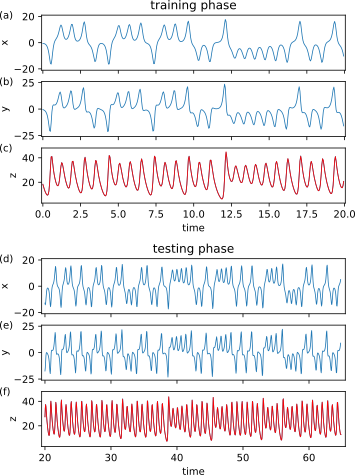
\includegraphics{figures/nvar-infer-lorenz}
  \caption{(a) -- (c) The Lorenz '63 system (blue) during the NVAR
    training. After the NVAR is trained, it is re-used on the
    training signal to produce the training output (c, red). (d) --
    (f) The Lorenz '63 system during NVAR testing, with the NVAR
    output. In both cases, the NVAR output (red) lies directly on top
    of the true Lorenz signal (blue).}
  \label{fig:nvar-infer-lorenz}
\end{figure}

I train this NVAR on $10$ different examples of the Lorenz '63
system, using $x$ and $y$ as the example input and $z$ as the example
output. Each training example is $20$ units of time. I then evaluate
the NVAR for $45$ units of time to produce a NRMSE $\epsilon$ as in
\cref{eq:nrmse}, and then average these errors over all $10$
trials. During evaluation, the NVAR has access to only $x$ and $z$,
and must produce an estimate of $z$. I then adjust $\alpha$ manually
to minimize this error. This whole process, training the NVAR $10$
different times and evaluating the error, takes only a few seconds on
a modern computer even with a poorly-optimized implementation.

I find this NVAR has a NRMSE of $1.75\mp0.3\times10^{-2}$ on this
inference task, using the ridge parameter $\alpha = 0.05$. An example of the NVAR during a
single training and testing trial is shown in
\cref{fig:nvar-infer-lorenz}.

\section{Forecasting Lorenz '63}

For this task, I use an NVAR in forecasting mode to do system
forecasting for the Lorenz '63 system. That is, I train the NVAR to use all
three state variables $x$, $y$, and $z$ to perform next-step-ahead
prediction of the Lorenz system in \cref{eq:lorenz}. Unlike for the inference task, once
the NVAR is in forecast mode it no longer has an external driving
input and runs autonomously. In analogy to other discrete-time integration algorithms, the choice of time step
$\Delta t$ has a stronger effect on forecasting than inference. Too
small a time step is wasted effort, and too large risks
inaccuracy. Here, I use a time step of $\Delta t = 0.025$, which results in about $40$ steps per Lyapunov period.

For this forecasting task I use only $2$ taps, $\tau_0 = 0$ and
$\tau_1 = 1$. This effectively gives the NVAR access to the current
value of the input as well as its derivative, and I find this
entirely sufficient for the forecasting task.
I use the quadratic nonlinearity with constant term described
in \cref{eq:quadratic-nvar-const}. With 2 taps and 3 input dimensions, the nonlinear output
of $\bm{g}_\text{n}$ has $1 + 6 + 21 = 28$ components, and so $W_\text{out}$ has
dimension $3 \times 28$.

Again, I train this NVAR on $10$ different examples of the Lorenz '63
system, each time training on $10$ units of time. I then evaluate the
NVAR by performing an autonomous forecast for one Lyapunov period to
calculate a NRMSE $\epsilon_1$, as in \cref{eq:nrmse}, and then
average this over the $10$ trials to produce $\tilde{\epsilon}$ in
\cref{eq:nrmse-avg}.

\begin{figure}
  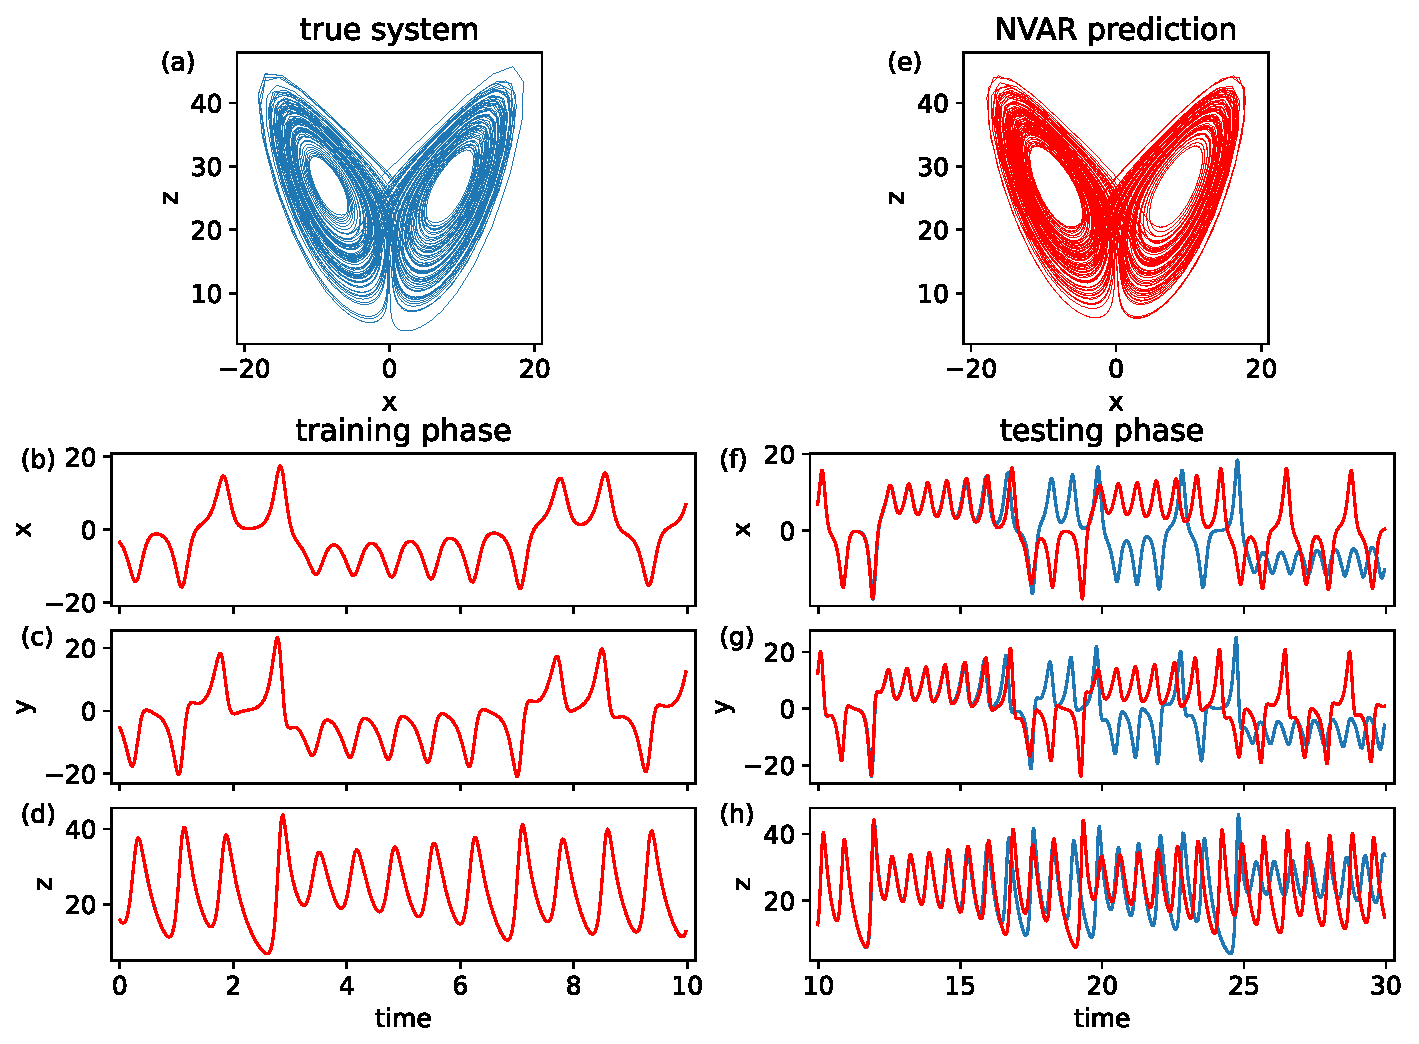
\includegraphics[width=\textwidth]{figures/nvar-predict-lorenz}
  \caption{The true Lorenz attractor (a) and NVAR predicted attractor
    (e) for a single training trial. (b) -- (d) True Lorenz system
    (blue) during training overlaid with NVAR output (red) calculated
    after training is complete. (f) -- (h) True (blue) and NVAR
    forecasted output (red). The NVAR shows good agreement with the
    true system as far as $5$ Lyapunov periods in to the autonomous
    forecast.}
  \label{fig:nvar-predict-lorenz}
\end{figure}

The performance of this NVAR during a single training trial is shown
in \cref{fig:nvar-predict-lorenz}. A long autonomous forecast from the
NVAR produces an attractor that shows qualitative agreement with the
true Lorenz attractor, and produces a NRMSE over one Lyapunov period
of $4.51\pm0.85\times10^{-3}$ using $\alpha = 2.5\times10^{-6}$, about
five times better than the ESNs described in
\cref{tab:lowk-lorenz-results}. This NVAR performs better than the
ESNs despite the fact that it is simpler to describe and implement,
does not require lengthy optimization, and trains at least an order of
magnitude faster. The training data used for the NVAR is also very
light: only $10$ units of time, corresponding to $400$ points at this
time step, is sufficient to train the NVAR.

\subsection{$z$ Return Map}

The $z$ variable of the Lorenz '63 system has a functional relation
between successive local maxima. This is demonstrated visually by
finding the local maxima $z_i$ of $z$, and then plotting $z_i$ with
respect to $z_{i+1}$ \cite{lorenz1963}. This \emph{return map} neatly
summarizes the long-term behavior of the $z$ variable, and comparing
two such maps provides a quick way to qualitatively compare two
systems. This comparison has been used previously to verify that a
trained RC can replicate the Lorenz '63 dynamics~\cite{pathak2017}.

In many ways, this comparison is similar to the visual inspection of the
reproduced attractor in \cref{fig:nvar-predict-lorenz}. However, the
return map is a simpler shape and is much more sensitive to error
than the attractor itself, even when comparing two maps by eye. Indeed,
the return map is so sensitive that it depends the specific integrator
used to find the true Lorenz '63 solution. Here, I use an explicit
Runge-Kutta 3(2)\cite{dormand1980} integrator for both the Lorenz '63
and double-scroll systems.

The values of the maxima in the discrete-time solutions for both the
NVAR and Lorenz '63 system depend on the time step $\Delta t$ used for
integration, as the true maximum may be achieved in between the
discrete time steps. To better reproduce the true Lorenz '63 return
map, and to reduce the effect $\Delta t$ has on the NVAR return map,
I interpolate the $z$ solutions by using a degree-$4$ spline. The
local maxima are then found on this interpolated spline~\cite{dierckx1995}.

\begin{figure}
  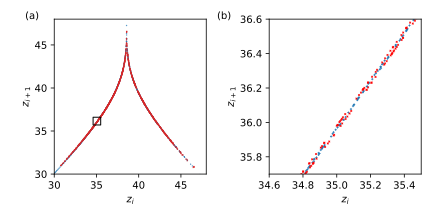
\includegraphics{figures/nvar-lorenz-rmap}
  \caption{(a) The $z$ return map of the Lorenz '63 system (blue $+$)
    overlaid with the $z$ return map of the NVAR forecast (red
    $\times$). The NVAR reproduces the long-term dynamics of the $z$
    variable accurately enough at this scale that it is difficult to
    see the true return map underneath. (b) Detail of the region
    marked in (a). At this scale, it is possible to see the small
    difference between the true and predicted return maps.}
  \label{fig:nvar-lorenz-rmap}
\end{figure}

\Cref{fig:nvar-lorenz-rmap} shows the return maps for both the true
Lorenz system and the NVAR. Qualitatively, there is good agreement
between the two. The NVAR return map almost completely obscures the
true Lorenz return map at this scale. Upon close inspection, I see
that the NVAR return map does not line up precisely with the true
return map. This can be improved by extending the training time of the
NVAR, but the difference between the two return maps is already small
even when the NVAR is trained for only $10$ units of time.

As with the attractor comparison, a quantitative measure of return map
similarity would be a strong candidate for replacing the flawed NRMSE
measure.

\subsection{Fixed Points}

For a more quantitative measure of how well the NVAR learns the
dynamics of the Lorenz system, I calculate the fixed points of the
trained NVAR and then find their distance to the true Lorenz fixed
points. By setting the derivatives in \cref{eq:lorenz} to zero, I
find three fixed points of the Lorenz system located at
\begin{align}
  [x, y, z] &= [0, 0, 0], \\
            &= [\pm \sqrt{\beta(\rho - 1)}, \pm \sqrt{\beta(\rho - 1)}, (\rho - 1)].
\end{align}

% fsolve, 'hybr' method, "Powell hybrid method"
% More, Jorge J., Burton S. Garbow, and Kenneth E. Hillstrom. 1980. User Guide for MINPACK-1.
To find the fixed points of the NVAR system, I perform a trial
single-step forecast with a constant past history, and use a
root-finding algorithm to find the specific values of past history
that result in an unchanged forecast. This root-finding algorithm is
used three times, using the three true Lorenz fixed points as initial
guesses.

To allow easy comparison of the accuracy of these fixed points with
other systems, I calculate the distance between this fixed points in
a uniformly scaled space where the Lorenz63 system has unit
variance. For this trained NVAR, the distance from the zero fixed point
is $1.2\pm1.4\times10^{-3}$, and the distances between the predicted
and true positive and negative fixed points are
$11.6\pm3.0\times10^{-4}$ and $7.4\pm1.5\times10^{-4}$, respectively.

The NVAR shows good agreement on the zero fixed point, as the variance
caused by different training windows overlaps with the true
location. The other two fixed points are consistently offset from the
truth. However, in all three cases, the fixed points lie within
approximately $0.1\%$ of the true location, despite the fact that the
training data does not include any of these points.

\subsection{Output Weights}

The particular choice of nonlinearity $\bm{g}_\text{n}$ for this task
completely includes all terms on the right hand side of the Lorenz
system in \cref{eq:lorenz}. That is, the Lorenz system is described by
a polynomial of degree $2$, and the choice of $\bm{g}_\text{n}$ allows
the NVAR to describe \emph{any} polynomial of degree $2$. This raises
a legitimate question: is the NVAR simply performing so well because
it was equipped ahead of time with the perfect tools?

\begin{figure}
  % FIXME fix labels \Delta t also 1 (also (a) not a) for other plots)
  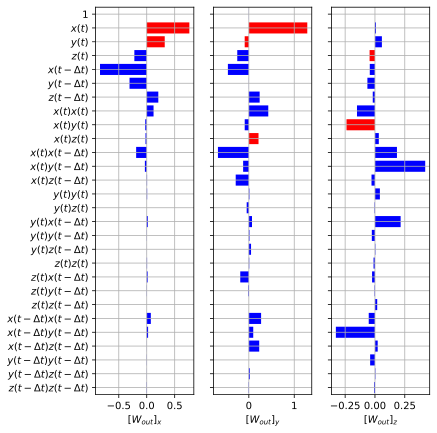
\includegraphics{figures/nvar-predict-lorenz-wout}
  \caption{Weights in the matrix $W_\text{out}$ for the NVAR trained
    for Lorenz system forecasting. Terms that appear directly in the
    Lorenz system (\cref{eq:lorenz}) are in red. There does not appear
    to be any correlation between a large weight in the NVAR output,
    and presence in the Lorenz equations.}
  \label{fig:nvar-predict-lorenz-wout}
\end{figure}

One way to allay these concerns is to look at other non-polynomial
systems, as in the next few sections. However, even with the Lorenz
system I see that this is not the case by inspecting the trained
weight matrix $W_\text{out}$ in
\cref{fig:nvar-predict-lorenz-wout}. There are significant contributions
in the output from terms not present in the Lorenz equations. From
this I derive an interpretation: a trained NVAR is finding the best
possible one-step-ahead integrator it can find, given the example
input and the available terms in $\bm{g}_\text{n}$. When the time step
is large enough, a strictly linear prediction becomes more and more
inaccurate, and so the NVAR relies on the nonlinear and time-delayed
terms to make up the difference.

\section{Forecasting the Double-Scroll Circuit}

For this task, I will use an NVAR in forecasting mode to use all
three state variables $V_1$, $V_2$, and $I$ of the double-scroll
circuit described by \cref{eq:dscroll}. I use the same tap
delays $\tau_0 = 0$, $\tau_1 = 1$ as the Lorenz case, but I modify
the choice of nonlinearity.

Unlike the Lorenz system, the double-scroll circuit cannot be
described by a polynomial of degree $2$. Indeed, the double-scroll
equations are odd, and have full inversion
symmetry. As a result, even terms in the nonlinear function
$\bm{g}_\text{n}$ are not useful to the NVAR. In light of this, I use
a nonlinear function that includes all linear terms of the tap vector
$\bm{v}$ as well as all terms with degree $3$. That is,
\begin{equation}
  \bm{g}_\text{n}(\bm{v}) = \bm{v} \oplus \ceil{\bm{v} \otimes \bm{v} \otimes \bm{v}}.
\end{equation}
With $2$ taps and $3$ input dimensions, the output of
$\bm{g}_\text{n}$ has $6 + 56 = 62$ components, and so $W_\text{out}$
has dimension $3 \times 62$.

The Lyapunov time of the double-scroll circuit is roughly $10$ times
longer than that of the Lorenz system. To ensure a fair comparison, I
extend the training time of the NVAR from $10$ to $100$ units to keep
the number of Lyapunov times covered by the training similar for both
cases. I also set $\Delta t = 0.25$, to ensure that both the Lorenz
and double-scroll cases use $400$ data points during training.

\begin{figure}
  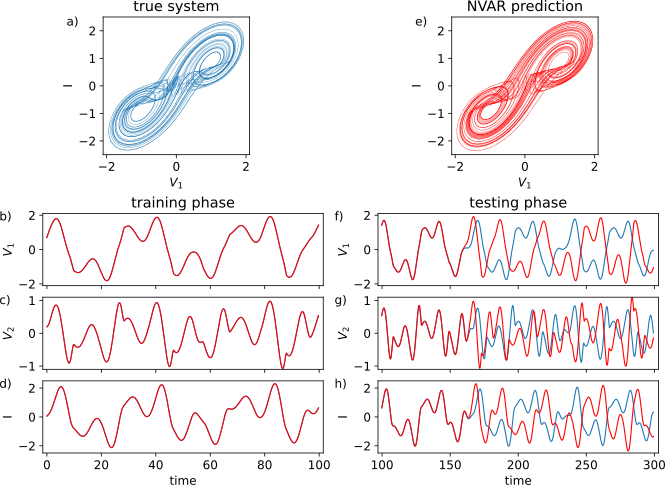
\includegraphics[width=\textwidth]{figures/nvar-predict-dscroll}
  \caption{The true double-scroll attractor (a) and NVAR predicted
    attractor (e) for a single training trial. (b) -- (d) True
    double-scroll system (blue) during training overlaid with NVAR
    output (red) calculated after training is complete. (f) -- (h)
    True (blue) and NVAR forecasted output (red). Again, the NVAR
    shows good agreement with the true system as far as $5$ Lyapunov
    periods.}
  \label{fig:nvar-predict-dscroll}
\end{figure}

Other than these modifications, the method for using the NVAR to
forecast the dynamics of this system proceeds exactly as for the Lorenz
system, training the NVAR on $10$ different examples of the
double-scroll circuit and then evaluating the NRMSE for one Lyapunov
period each. The performance of this NVAR during a single training
trial is shown in \cref{fig:nvar-predict-dscroll}.

Once again, a long autonomous forecast shows the NVAR can reproduce
the shape of the double-scroll attractor, and over one Lyapunov period
has an NRMSE of $2.15\pm0.63\times10^{-2}$ using $\alpha =
1.0\times10^{-3}$, about $1.5\times$ better than the ESNs
described in \cref{tab:lowk-resultsplus}.

\subsection{Fixed Points}

Again, I look for the fixed points of this trained NVAR and find
their distance to the true fixed points of the double-scroll circuit,
in a space uniformly scaled so that the double-scroll circuit has unit
variance. Setting the derivatives in \cref{eq:dscroll} to $0$
and solving yields the transcendental equation
\begin{equation}
  0 = \frac{V_1}{R_2}(R_1 - R_2 - R_4) + 2 R_1 I_r \sinh\left(\alpha V_1 \left(1 - \frac{R_4}{R_1}\right)\right).
\end{equation}
For the parameters I use, this yields three solutions for $V_1$. If
$V_1^+$ is the positive solution, this corresponds to three fixed points
at
\begin{align}
  [V_1, V_2, I] &= [0, 0, 0], \\
                &= [V_1^+, \pm V_1^+ R_4 / R_1, \pm V_1^+ / R_1].
\end{align}

Since my choice of $\bm{g}_\text{n}$ has only odd polynomial powers
and no constant term, it is symmetric about the origin and predicts
the zero fixed point exactly. The distance from the true positive
fixed point is $2.7\pm0.3\times10^{-3}$. Due to the inversion
symmetry, the negative fixed point is precisely the same
distance. Although the variance from repeated trials does not overlap
the true fixed points, they do lie within $0.3\%$ of the truth.

This NVAR performs well at short-term forecasting and fixed point
prediction, despite not having access to the infinite number of
polynomial terms in the expansion of the double-scroll equations. This
demonstrates a possible practical approach to NVAR design: keep adding
delay taps and higher polynomial terms to the nonlinear function
$\bm{g}_\text{n}$ until performance is acceptable. However, for NVARs
that require many taps or operate on high-dimensional inputs, this
very quickly leads to an explosion in the number of weights trained in
$W_\text{out}$, and consequently a huge increase in training time. In
the next section, I will explore how careful use of tap spacing can
keep the number of taps required low.

\section{Forecasting Mackey-Glass}

% FIXME how integrated

For this task, I will again use an NVAR in forecasting mode, this time
using the single Mackey-Glass state variable $u$ (in
\cref{eq:mackey-glass}) as input, with $\Delta t = 0.2$. For this
system, using two adjacent taps for the NVAR as in the previous
examples is insufficient, as the Mackey-Glass system behavior depends
strongly on both the value of $u(t)$ as well as $u(t - 17)$. One way
to access this value in the NVAR is to add taps at every time step
until they reach $t = 17$, resulting in $85$ total taps. Even with only a
quadratic output, this requires training a $W_\text{out}$ with
dimension $1 \times 3741$. This cost can be avoided by increasing the
time step $\Delta t$, thus reducing the total number of taps, but this
solution comes with the cost of a much more granular prediction.

Another way to access the value at $u(t-17)$ is to use only two taps,
placed at $\tau_0 = 0$ and $\tau_1 = 17 / \Delta t$, which is the
method I use here. I also use a nonlinear function
$\bm{g}_\text{n}$ that includes the constant, linear, quadratic, and
cubic terms constructed from the tap vector $\bm{v}$,
\begin{equation}
  \bm{g}_\text{n}(\bm{v}) = 1 \oplus \bm{v} \oplus \ceil{\bm{v} \otimes \bm{v}} \oplus \ceil{\bm{v} \otimes \bm{v} \otimes \bm{v}}.
\end{equation}
With $2$ taps and $1$ input dimension, the output of $\bm{g}_\text{n}$
has $1 + 2 + 3 + 4 = 10$ components, and so $W_\text{out}$ has
dimension $1 \times 10$.

The Lyapunov time of the Mackey-Glass system is roughly $100$ times
longer than that of the Lorenz system. However, I find that a
relatively fine step size $\Delta t = 0.2$ is required for the NVAR to
learn the system, corresponding to $500$ points per Lyapunov period. I train this NVAR for $1000$ units of time,
corresponding to $5000$ data points total. Though this is many more
discrete data points, it covers about $10$ Lyapunov times, comparable
to the training time used for the other systems.

This NVAR is much more data hungry than the previous examples,
requiring more training data to produce an acceptable result. This may
be due to the wide tap spacing: values at $u(t - 17)$ are less
correlated to $u(t)$, while $u(t - \Delta t)$ is more correlated, and
so the NVAR needs more data to see every relevant combination of
values at the taps.

\begin{figure}
  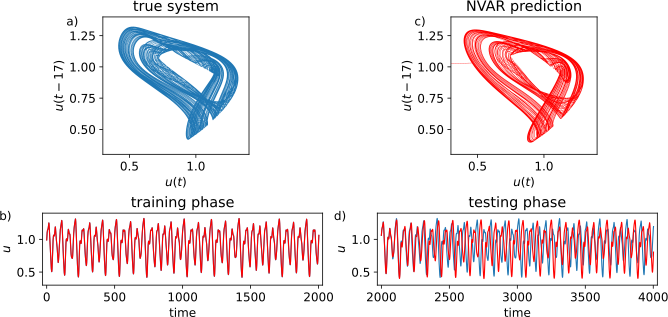
\includegraphics[width=\textwidth]{figures/nvar-predict-mackey-glass}
  \caption{The true Mackey-Glass attractor (a) and NVAR predicted
    attractor (c) for a single training trial. (b) True Mackey-Glass
    system during training overlaid with NVAR output (red) calculated
    after training is complete. (d) True (blue) and NVAR forecasted
    output (red). Here, the NVAR shows good agreement with the true
    system as far as $2$ Lyapunov periods.}
  \label{fig:nvar-predict-mackey-glass}
\end{figure}

Other than these modifications, the methodology for training and
evaluating the NVAR is exactly as for the other two systems. The
performance of this NVAR during a single training trial is shown in
\cref{fig:nvar-predict-mackey-glass}. Over one Lyapunov period, this
NVAR has a NRMSE of $1.4\pm0.2\times10^{-1}$ with $\alpha =
9\times10^{-2}$.

The long autonomous forecast of the NVAR shares important features
with the true attractor, most notably the gap between the
bands. However, it does not reproduce the shape of the heel in the
upper-left corner very well, and this is reflected in the high NRMSE.

% FIXME cite kernel trick

The shape of this heel can be better reproduced by including
higher-order terms in the nonlinear function
$\bm{g}_\text{out}$. However, it is not possible to do this with
monomial terms as I have been doing without dramatically increasing
the training time of $W_\text{out}$. It may be possible to instead add
nonlinear terms to $\bm{g}_\text{out}$ with an infinite power series,
such as $e^{v_iv_j}$ or $\sinh{v_i}\cosh{v_j}$. This would provide
access to high-order nonlinearity without a corresponding large increase in training
time. This is one important avenue for future research, and this
Mackey-Glass forecasting example demonstrates that cubic terms are not
completely sufficient for accurate forecasts. Nonetheless, the cubic
NVAR used here shows promising performance from a simple model.

% FIXME fixed point?

\section{Conclusion}

In this chapter, I have demonstrated the NVAR approach on two classic
RC problems: state inference and system forecasting. I have shown that
NVARs can solve these problems as well, or in some cases better, than
the RC approach, despite the simplicity of the NVAR method. At the
same time, I have resolved the remaining questions raised in
\cref{ch:nvar}: NVARs remain useful even with only a handful of
time-delay taps, and a simple extension of the nonlinear function
$\bm{g}_\text{n}$ to include higher-order monomial terms is sufficient
in many cases.

The Mackey-Glass forecasting task sits at the very edge of this simple
technique. It shows that a low number of time-delay taps remains
sufficient even in systems with long, built-in time delays. However,
it also demonstrates that a cubic nonlinearity is not sufficient to
reproduce the precise shape of the Mackey-Glass attractor. To move
forward with the NVAR technique, the nonlinear function
$\bm{g}_\text{n}$ will need to include much higher-order terms, and it
will need to do so without the exponential increase in training time
associated with adding more monomial terms to the output.

% FIXME kernel trick here too
